%==============================================================================
% Section 5: chi-universality across diagnostic and reduced-orbit levels
%==============================================================================
\section{$\chi$-universality across diagnostic and reduced-orbit levels}
\label{sec:bridge}

\subsection{Two independent appearances of $\chi$}
\label{sec:bridge:two_appearances}

The central claim of this paper is the bridge result that two independent
computations converge on the same scalar $\chi$.

\begin{table}[H]
\centering
\begin{tabular}{lll}
\toprule
Level & Equation & Derivation route \\
\midrule
Diagnostic     & $\Ctop=-9\chi$        & template extraction from raw $\PintMX$ \\
Reduced orbit  & $\dot q^{2}+\chi=0$   & vacuum orbit atlas on the auxiliary shell \\
\bottomrule
\end{tabular}
\caption{$\chi$-universality summary.}
\label{tab:chi_universality_summary}
\end{table}

\begin{figure}[H]
  \centering
  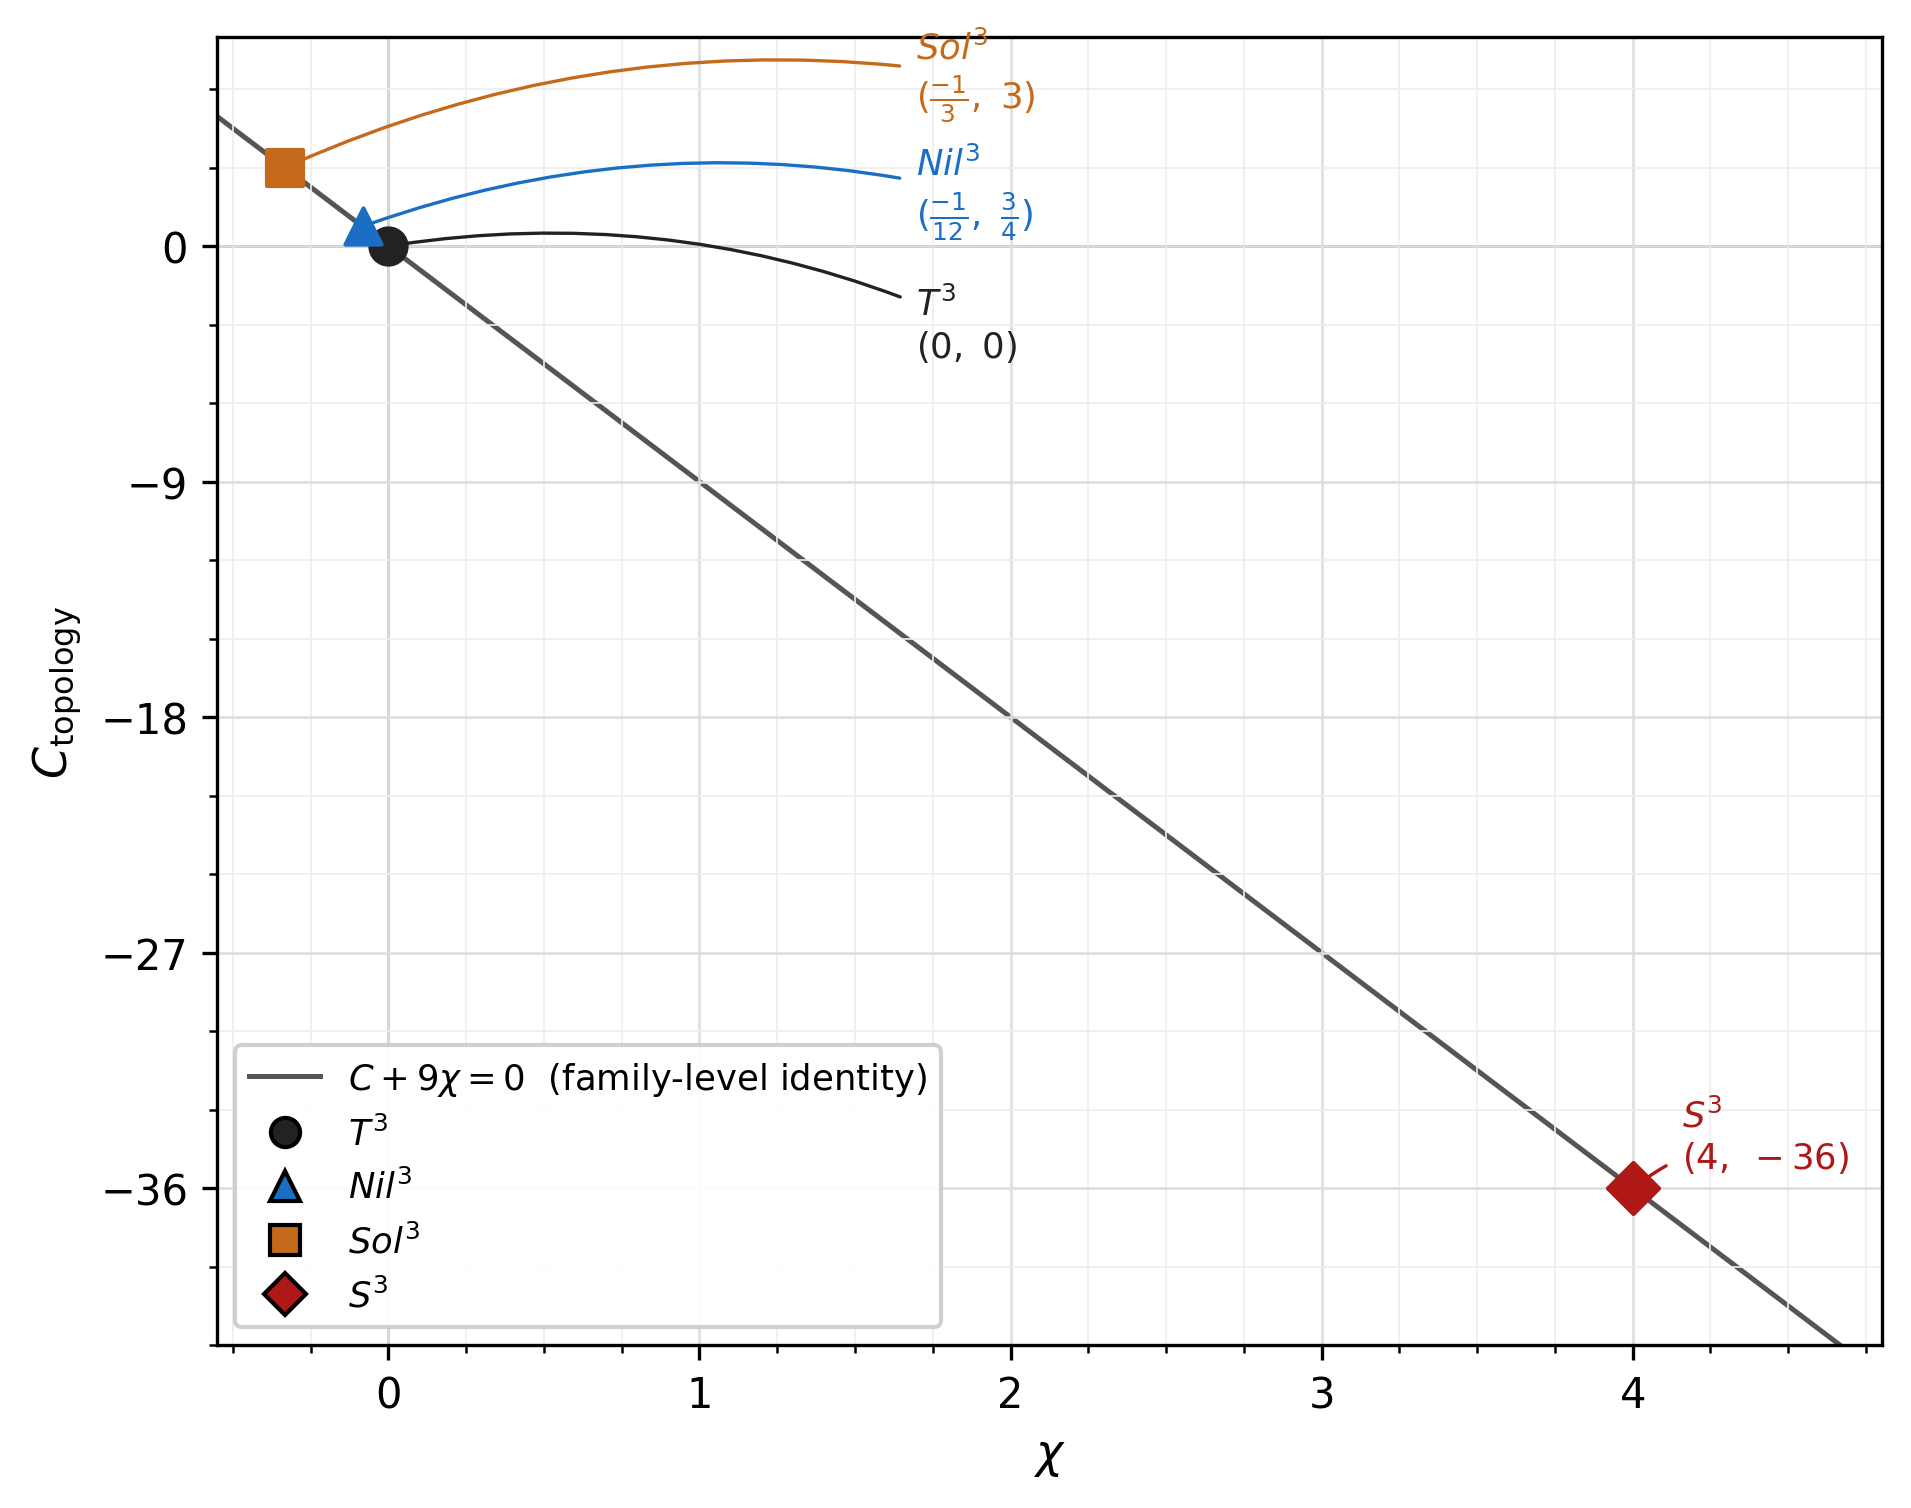
\includegraphics[width=0.9\textwidth]{figures/fig02_chi_bridge_line.png}
  \caption{Diagnostic bridge: the $\Ctop=-9\chi$ line.  The horizontal axis
    is $\chi$ (derived independently from the LC spatial curvature) and the
    vertical axis is $\Ctop$ (extracted from the raw symbolic expression of
    $\PintMX$ by template fitting, without reference to $\chi$).  The four
    points $\Tthree$, $\Nilthree$, $\Solthree$, $\Sthree$ all lie exactly on
    the line $\Ctop+9\chi=0$.  The line is the graphical representation of
    the family-level identity of Section~\ref{sec:bridge:family}; the four
    points are its specialisations.  \emph{Scope}: a family-level identity
    within the LZ-native isotropic $\MX$ sector; $\PintMX$ is an
    internal-pair diagnostic, not a true Pontryagin density.}
  \label{fig:chi_bridge_line}
\end{figure}

The independence of these two quantities deserves emphasis.  As stated in
Section~\ref{sec:pchannel:Pint}, $\Ctop$ is a coefficient extracted from the
raw symbolic expression of $\PintMX$ without reference to $\chi$.  In
contrast, $\chi$ is derived independently from the spatial-curvature sector
as
\begin{equation}
  \chi = \frac{{}^{(3)}R\, q^{2}}{6}.
\end{equation}
Neither computation takes the other quantity as an input, so the relation
$\Ctop = -9\chi$ is not a rephrasing of a definition but the bridge result
between two independent computational routes.

\subsection{Five-parameter family-level identity}
\label{sec:bridge:family}

Over the full five-parameter LZ-native isotropic family of
Section~\ref{sec:setup:chi}, the family-level expression for $\Ctop$ is
\begin{equation}
  \Ctop
  = \frac{3}{4}\,\Disc
  = \frac{3}{4}\!\left(a^{2}-2ab-2ac+b^{2}-2bc+c^{2}
    +4u^{2}+4uv+4v^{2}\right),
\end{equation}
and since $\chi=-\Disc/12$,
\begin{equation}
  \Ctop + 9\chi
  = \frac{3\Disc}{4} - \frac{9\Disc}{12} = 0
\end{equation}
holds as an exact symbolic identity.  This identity is a structural identity
over the entire five-parameter family, not just at the four specific
numerical values of the topologies; the algebraic core is given in
Appendix~\ref{app:B}.

\subsection{Distinguished topology loci}
\label{sec:bridge:loci}

The four topologies are not arbitrary sample points of the five-parameter
family but are located at structurally distinguished loci
(Table~\ref{tab:distinguished_loci}).

\begin{table}[H]
\centering
\resizebox{\linewidth}{!}{%
\begin{tabular}{lcrrll}
\toprule
Topology & $(a,b,c,u,v)$ & $\chi$ & $\Ctop=-9\chi$ & Structural locus & paper~IV echo \\
\midrule
$\Tthree$   & $(0,0,0,0,0)$  & $0$    & $0$  & origin                          & none \\
$\Nilthree$ & $(0,0,-1,0,0)$ & $-1/12$ & $3/4$ & single class-A axis            & uniaxial \\
$\Sthree$   & $(4,4,4,0,0)$  & $4$    & $-36$ & isotropic class-A diagonal     & triaxial \\
$\Solthree$ & $(0,0,0,1,-1)$ & $-1/3$ & $3$  & balanced class-B diagonal pair & biaxial \\
\bottomrule
\end{tabular}%
}
\caption{Distinguished topology loci and paper~IV echo.}
\label{tab:distinguished_loci}
\end{table}

The ``paper~IV echo'' column records an interpretive correspondence with
the KK Higgsing response dictionary of paper~IV (none / uniaxial / triaxial
/ biaxial); details are given in
Section~\ref{sec:discussion:paper04echo}.

\begin{figure}[H]
  \centering
  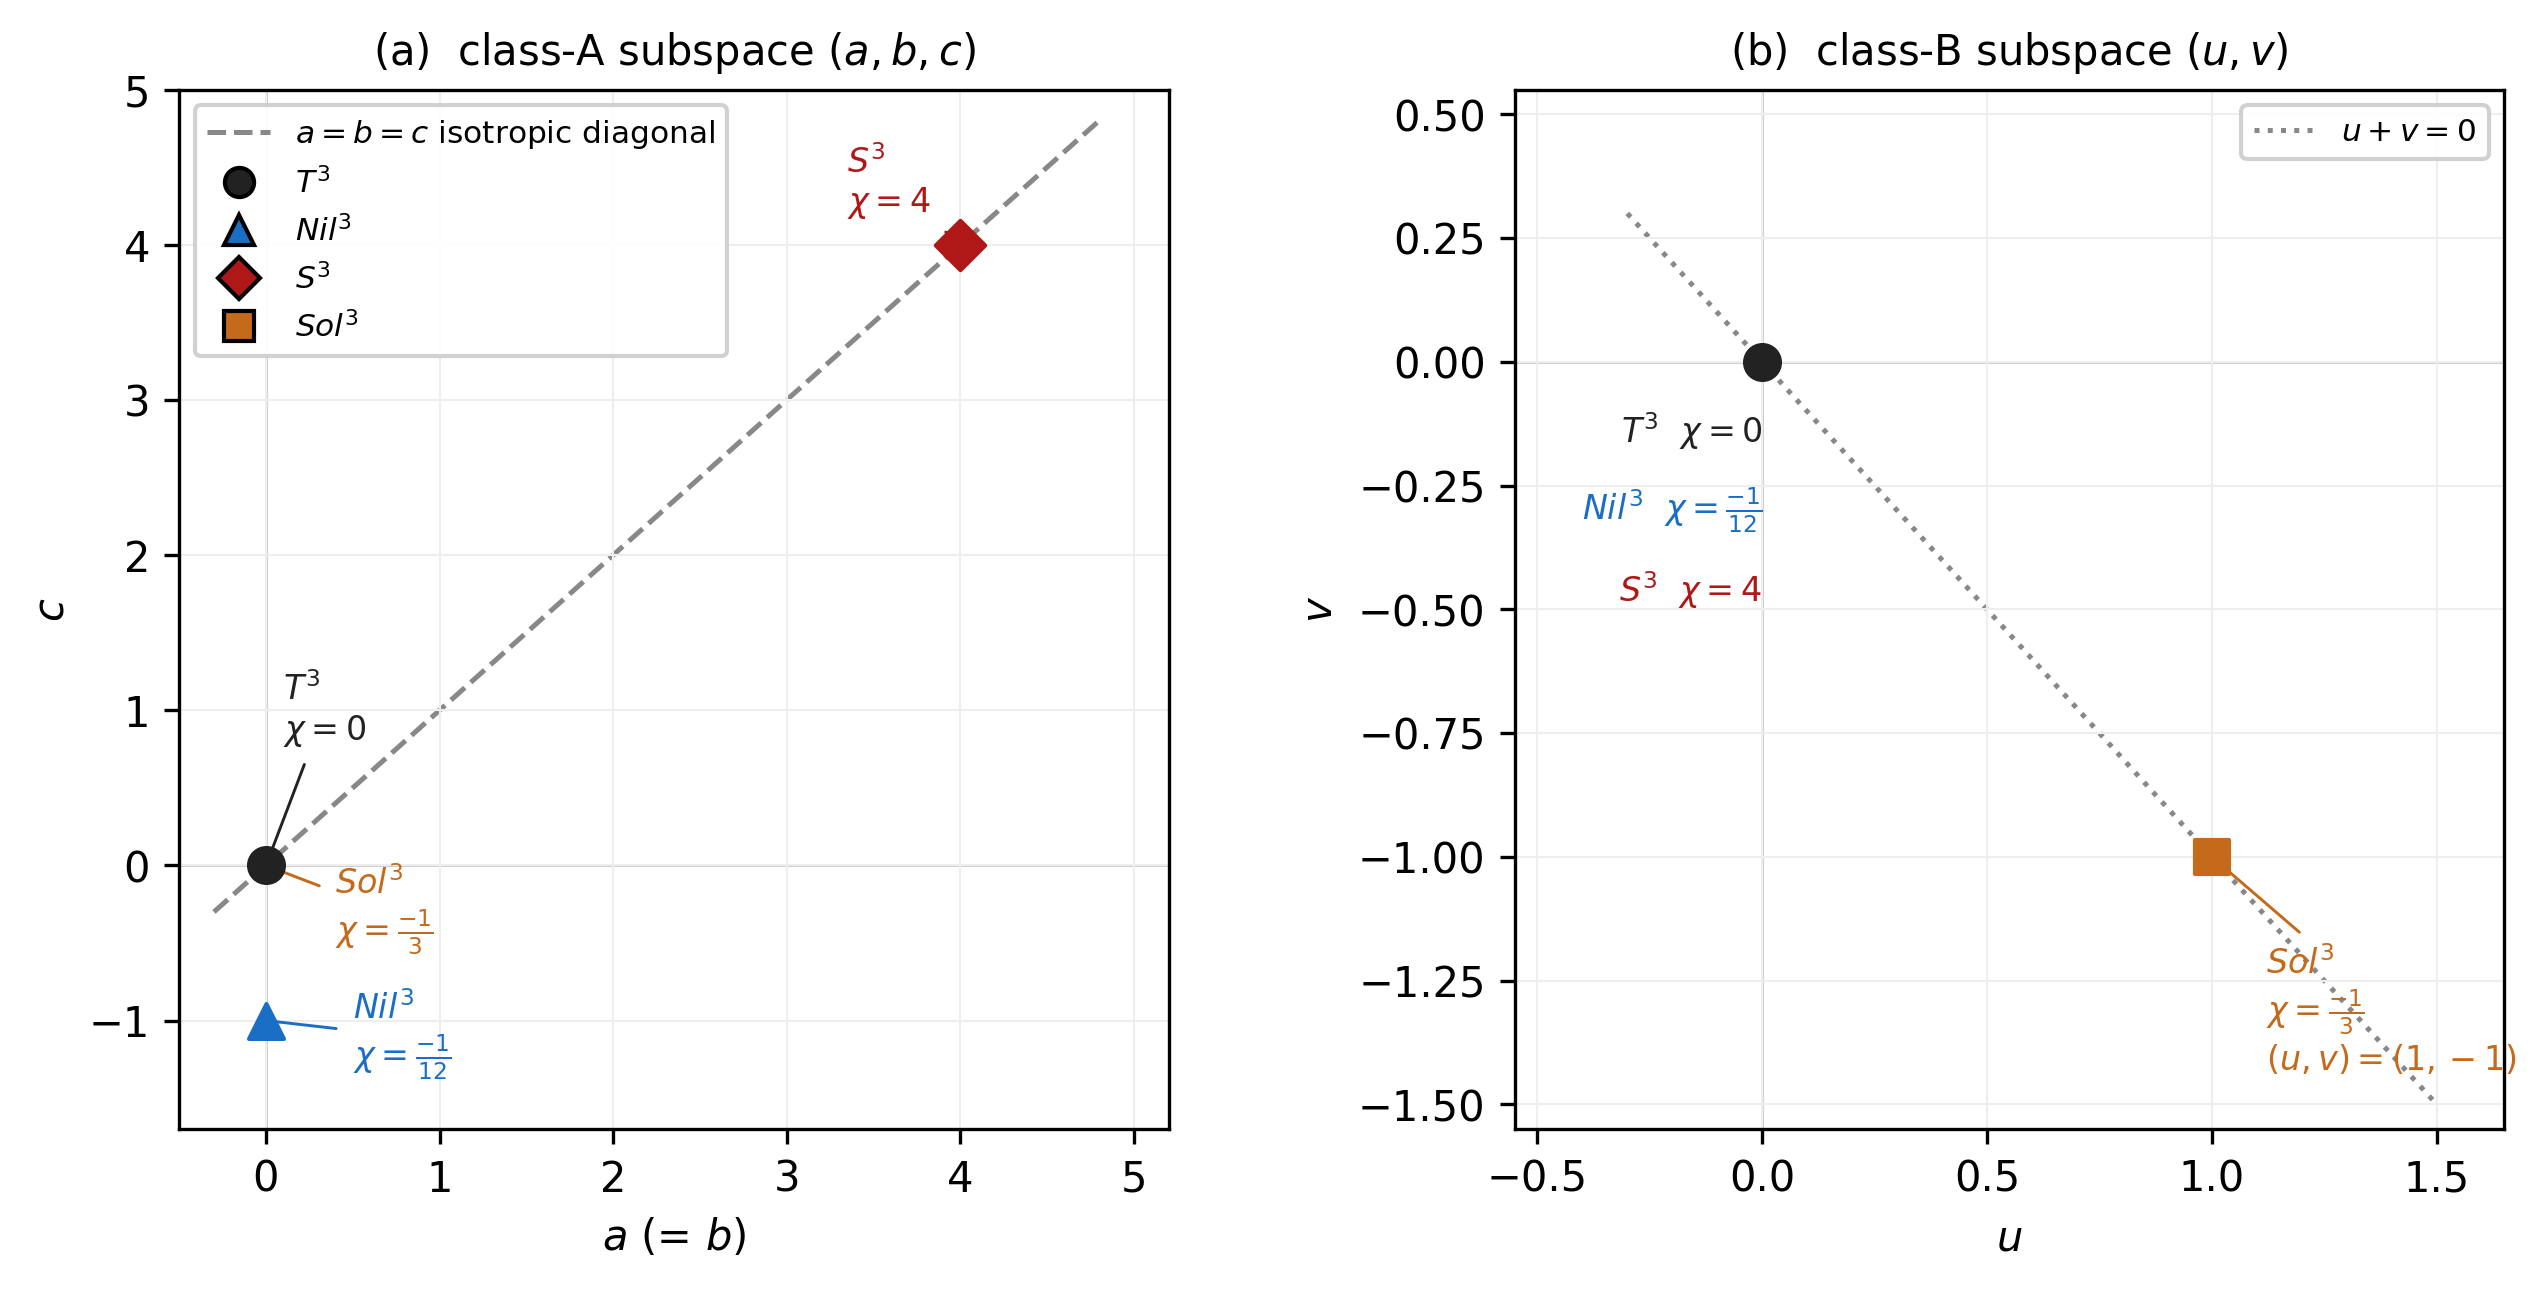
\includegraphics[width=1.0\textwidth]{figures/fig03_loci_diagram.png}
  \caption{Distinguished loci in the five-parameter family
    $(a,b,c,u,v)$.  \textbf{(a) class-A subspace $(a,b,c)$}: all topologies
    lie in the plane $b=a$ and are shown in the $(a,c)$ coordinates.
    $\Tthree$ and $\Solthree$ sit at the class-A origin, $\Nilthree$ on a
    single axis, and $\Sthree$ on the isotropic diagonal $a=b=c$ (dashed).
    \textbf{(b) class-B subspace $(u,v)$}: $\Tthree$, $\Nilthree$, and
    $\Sthree$ collapse to the $u=v=0$ origin, while $\Solthree$ sits at the
    balanced pair $(u,v)=(1,-1)$ on the line $u+v=0$ (dotted).  The four
    points are structurally distinguished loci of the family, not arbitrary
    samples.  \emph{Caveat}: the ``paper~IV echo'' label indicates a
    structural resonance with the paper~IV KK Higgsing dictionary, not an
    identification of the underlying mechanism or theorem
    (see Section~\ref{sec:discussion:paper04echo}).  The present family is
    the LZ-native isotropic $\MX$ family, not a full-theory universal
    family.}
  \label{fig:loci_diagram}
\end{figure}

The scope of $\chi$-universality is restricted to the LZ-native isotropic
$\MX$ reduced sector of this paper.  Extensions to full-theory
universality, arbitrary anisotropic EOM, or matter-coupled sectors are not
claimed here.
